\section{Introduction}
\label{sec:Introduction}

This analysis note presents the measurement of the polarizations of the \jpsi and \psip mesons promptly and non-promptly produced in proton-proton collisions at $\sqrt{s} = 13$\,\TeV, on the basis of data collected in 2017 and 2018 by the CMS experiment. This is a much larger sample than the one collected in 2011, at 7\,\TeV, which was used for the previous CMS measurement of the prompt \jpsi and \psip polarizations. Besides the obvious improvement in the statistical uncertainties, the Run~2 sample allows us to probe a much broader \pt range, extending to \pt values well in excess of those reached before.

\subsection{Previous CMS quarkonium polarization analyses}

The work described in this document represents one more step in a series of CMS measurements 
of the polarizations of quarkonium states.
We started with the measurement of the polarizations of the Upsilon states, 
as a function of \pt and in two rapidity ranges,
using the 7\TeV pp data collected by CMS in 2011 (analysis BPH-11-023)~\cite{bib:BPH-11-023}, 
a work described in detail in the analysis note AN-2012/140.
This measurement implied the development of an original analysis framework, 
explained in the analysis note AN-2011/535~\cite{bib:AN-2011/535}.
Once this first step was completed, the analysis team moved to the BPH-13-003 analysis, 
the measurement of the polarizations of the 
\jpsi and \psip states promptly produced in 7\TeV pp collisions~\cite{bib:BPH-13-003},
a work described in the analysis note AN-2013/016.
This second work had the extra challenge of ensuring that the non-prompt charmonia,
resulting from decays of B hadrons, could be properly removed from the signal sample,
through the simultaneous analysis of the dimuon mass and pseudo-proper lifetime.
The effort that went into these two analyses gave birth to two more publications:
the measurement of the \jpsi and \psip cross sections in pp collisions at 7\TeV 
(BPH-14-001)~\cite{bib:BPH-14-001},
and the measurement of the polarizations of the Upsilon states as a function of 
the multiplicity of charged tracks produced in the pp collisions 
(HIN-15-003)~\cite{bib:HIN-15-003}.

The analysis BPH-13-001 represented one more step in increasing complexity:
the measurement of the polarizations of the \chicOne and \chicTwo mesons 
promptly produced in proton-proton collisions at $\sqrt{s} = 8$\TeV~\cite{bib:BPH-13-001}.
This work is described in detail in the analysis note AN-2019/045.
The difficulty of discriminating the prompt and non-prompt contributions
was solved through the analysis of the dimuon pseudo-proper lifetime distribution,
following an improved version of the formalism previously used in the BPH-13-003 work.
The bigger challenge was the identification of an event sample of \chic candidates,
reconstructed by combining the dimuon emitted in the \jpsi decay with a photon
produced in the radiative \chic decay: $\chic \to \jpsi \gamma$.
The photon was exclusively detected using conversions to $e^+e^-$ pairs,
reconstructed in the CMS silicon tracker,
which provides a \chic mass measurement with sufficient resolution to discriminate the
\chicOne and \chicTwo components.
This is a crucial aspect of the analysis, in view of reaching an independent measurement of 
the polarizations of the two mesons.
The technique used for the detection of photon conversions 
had been previously developed in CMS and was at the basis of two CMS publications,
reporting the cross-section ratios of P-wave states: 
$\chicTwo / \chicOne$ (BPH-11-010)~\cite{bib:BPH-11-010} and 
$\chibTwo / \chibOne$ (BPH-13-005)~\cite{bib:BPH-13-005}.

Along the way, four PhD theses have been prepared and defended, 
by Valentin Kn{\"u}nz~\cite{bib:ValentinPhD},
Ilse Kr{\"a}tschmer~\cite{bib:IlsePhD}, 
Chris Ferraioli~\cite{bib:ChrisPhD}, 
and Thomas Madlener~\cite{bib:ThomasPhD},
which constitute an exceptional source of detailed and pedagogical information, 
well suited for the ``interested readers".

\subsection{Brief overview of the analysis}

The analysis provides the polarizations of the \emph{prompt} and 
\emph{non-prompt} \jpsi and \psip mesons.
The prompt and non-prompt events are selected using the pseudo-proper lifetime observable.
Besides the directly produced component, the prompt \jpsi event sample includes 
``feed-down decays" of heavier charmonium states:
around 8\% of mesons produced in \psip decays and 
around 25\% produced in \chic decays~\cite{bib:Faccioli-feeddown}.
No such feed-down sources contribute to the \psip sample.
The non-prompt mesons are produced in (inclusive) decays of B mesons.

The measurement is, as in all the previous analyses, based on the 
analysis of the angular distributions of the dimuons
resulting from the decay of the quarkonium mesons.
The polarization extraction method used in this analysis uses the information
content of the dimuon mass distribution to separate the \jpsi signal contribution 
from the muon pairs resulting from other processes 
(mostly pairs of muons resulting from decays of uncorrelated heavy flavour mesons).
The 4-momentum vectors of the two muons, 
containing the spin alignment information of the decaying meson, 
are used to extract the anisotropy parameters $\lambda$ (see next section)
in each independent \pt bin.
Given that, as expected,
no rapidity-dependences have been seen in the previous measurements,
this analysis is made integrated over the dimuon rapidity window $|y| < 1.2$,
without splitting this (relatively narrow) mid-rapidity window into thinner bins.

The physics result is reported in the form of the polar anisotropy parameter 
in the centre-of-mass helicity frame, $\lth^{\rm HX}$.
The azimuthal anisotropy is also studied, essentially to confirm that, 
in the HX frame, it can be neglected.
Residual azimuthal anisotropies are taken into account 
as a systematic uncertainty in $\lth^{\rm HX}$.

\subsection{Physics motivation for a high-precision polarization measurement}

Vector particles (Z, W, Drell--Yan) are generally produced with maximal polarization. 
Even if for a given \pt, in a given frame, the polarization can be zero, 
there must always exist a kinematical domain and an ``optimal'' frame 
where it approaches maximal values. In fact, vector states are intrinsically polarized.

This statement can be presented in the form of a theorem 
(see Ref.~\cite{bib:Faccioli-PRL-FrameInv} for details):
for any subprocess producing a $J=1$ state 
$|V;J, J_z \rangle = a_{-1} |1, -1\rangle + a_{0} |1, 0\rangle + a_{+1} |1, +1\rangle$, 
there exists a quantization axis with respect to which the $J_z = 0$ component vanishes, 
which implies that $\lth = +1$ along that axis.
This is intuitively consistent with the classical expectation: 
a vector of modulus unity has always projection $\pm$1 along \emph{some} axis.

\begin{figure}[h]
\centering
\resizebox{0.6\linewidth}{!}{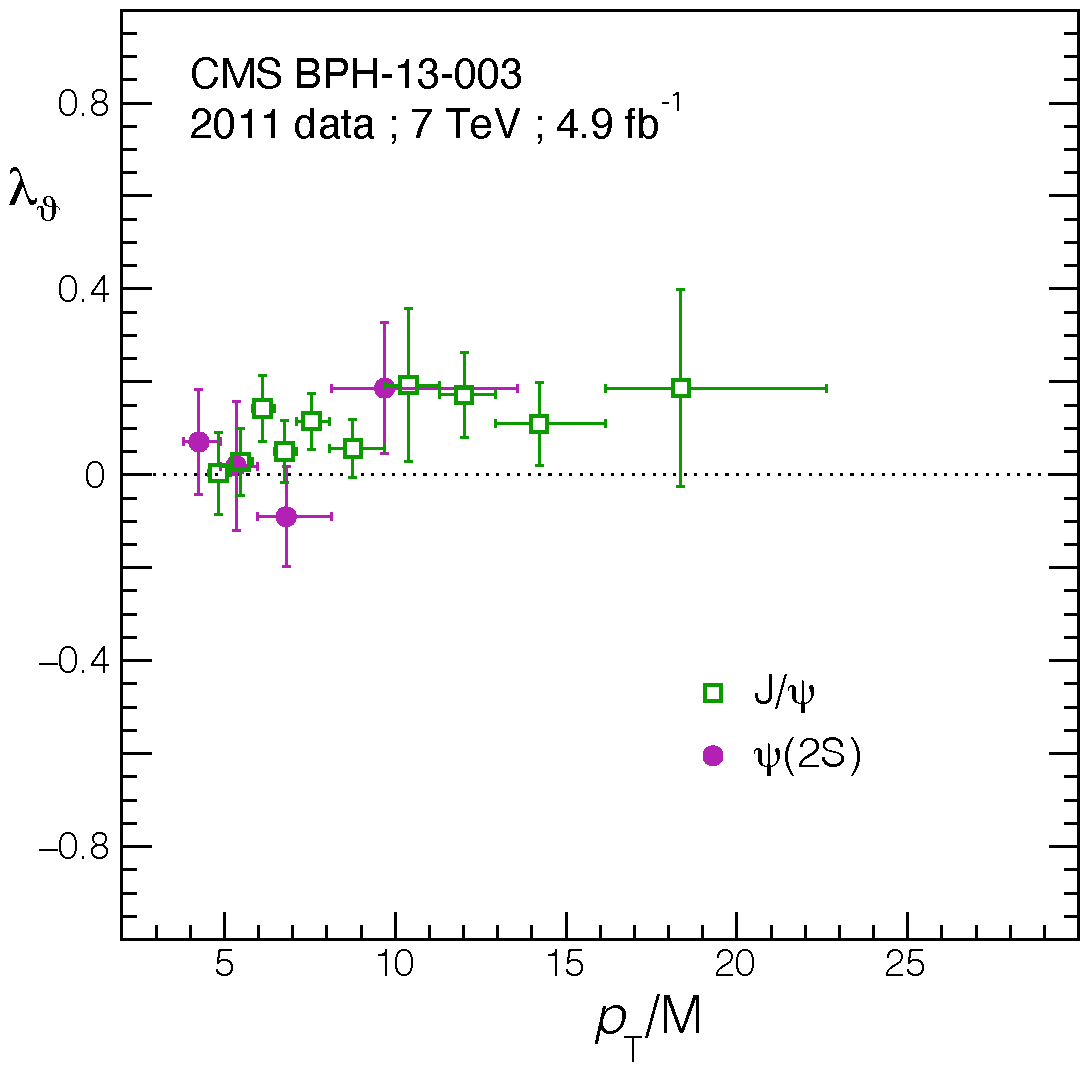
\includegraphics{Figures/chapter1/Jpsi_psi2S_pol.pdf}}
\caption{Polar anisotropy parameter, \lth, as a function of the quarkonium 
mass-scaled \pt, for the \jpsi and \psip promptly-produced in the
7\TeV pp collisions collected by CMS in 2011.}
\label{fig:BPH13003}
\end{figure}

Given this understanding, it is surprising to see that the BPH-13-003
results indicate that the \jpsi and \psip polarizations are close to zero, 
as illustrated in Fig.~\ref{fig:BPH13003}.
The only reasonable explanations are that we measure negligible polarizations 
because 1)~we are seeing the superposition of
several production subprocesses that, thanks to a ``fortunate coincidence", 
cancel each other, or 2)~we are seeing the result of a ``randomization step" that
completely smears away the initial strong polarization, so that we end up with 
almost isotropic dimuon angular decay distributions.

\begin{figure}[h]
\centering
\resizebox{0.5\linewidth}{!}{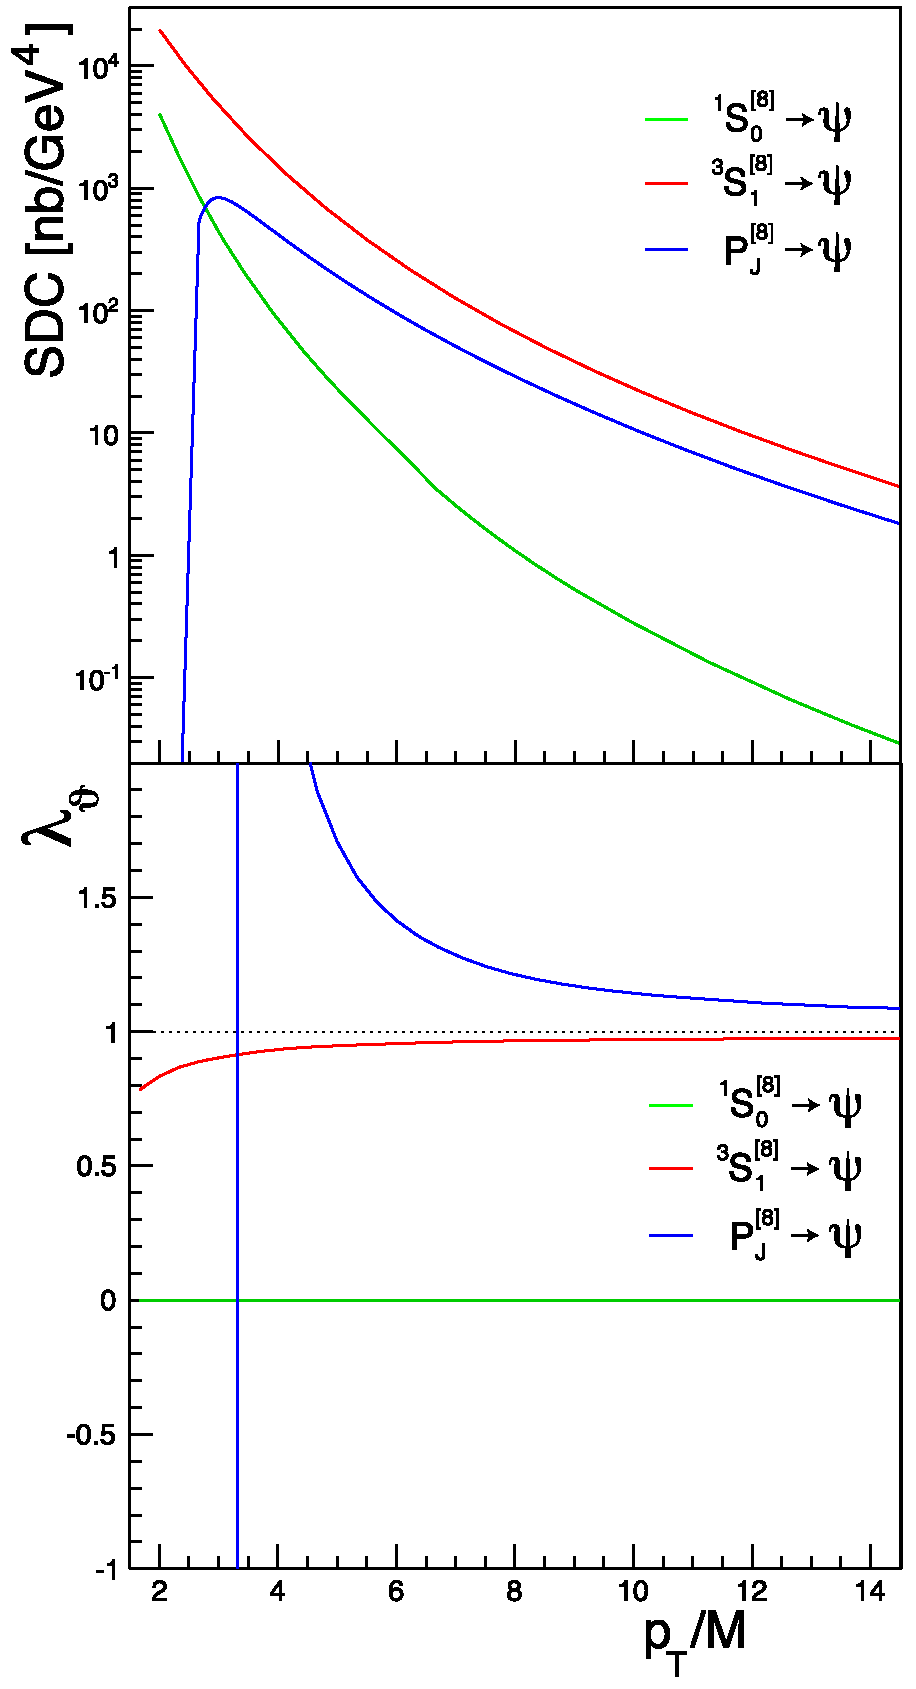
\includegraphics{Figures/chapter1/NRQCD_dists.pdf}}
\caption{Differential cross sections (``SDCs", top) and polarizations (\lth, bottom) of the three colour octets
expected to dominate \jpsi and \psip production in the NRQCD framework,
computed at NLO.}
\label{fig:NRQCD}
\end{figure}

This experimental observation does not match what one would naturally expect
in the context of the NRQCD theoretical approach. Indeed, within NRQCD, 
the \jpsi and \psip production should be dominated by three colour octet
terms (the colour singlet having a negligible contribution) of similar magnitude:
the $^1S^{[8]}_0$, $^3S^{[8]}_1$, and $^3P^{[8]}_J$ (pre-resonant) \ccbar states. 
As shown in Fig.~\ref{fig:NRQCD}, these three terms have rather different 
polarizations. The $^1S^{[8]}_0$ term leads to mesons that are intrinsically polarized 
along the \emph{unobservable} $^1S^{[8]}_0$-state direction, so that they look 
unpolarized, because of rotational smearing. Instead, the $^3S^{[8]}_1$ and 
$^3P^{[8]}_J$ octets produce strongly polarized quarkonia states, with the \lth
of the $^3S^{[8]}_1$ contribution being close to the maximum physical limit, $+1$,
and that of the $^3P^{[8]}_J$ term being even larger than that limit. 
With suitable relative weights, one can add the three terms so that the sum 
gives zero at a given \pt value but, as we can easily see by looking at the three 
very different curves shown on the bottom panel of Fig.~\ref{fig:NRQCD}, it is
not possible to reach a null sum over a broad \pt range, a conclusion that is in
contradiction with the seemingly flat measured patterns seen in Fig.~\ref{fig:BPH13003}.

However, the relatively poor precision of the measurements shown in Fig.~\ref{fig:BPH13003}
leave the door open to the possibility of non-flat trends, so that, for now, we can consider
the following three scenarios:
\begin{enumerate}
\item[1)] we are seeing an \emph{accidental} cancellation of the $^3S^{[8]}_1$ and 
$^3P^{[8]}_J$ terms in a narrow \pt domain, in which case a more precise measurement 
will reveal a non-flat trend;
\item[2)] we are in the presence of an exact degeneracy between the colour-octet terms,
at least as computed at NLO,
so that their sum is identical to the (unpolarized) $^1S^{[8]}_0$ term alone, 
in which case we would have to conclude that the NRQCD expansion is not a natural 
description of nature;
\item[3)] we are seeing that the $^1S^{[8]}_0$ term completely dominates over the other two, 
in which case we would have clear evidence showing that the NRQCD $v^2$ scaling 
hierarchy fails for charmonium production.
\end{enumerate}

The prompt \jpsi polarization measurement made using the 2017 and 2018 data samples,
reported in this AN,
is sufficiently precise to see if the trend of \lth with \pt is essentially flat or 
starts showing a significant slope at some \pt value. 
So, the main goal of this measurement is to evaluate if the pattern of \lth as a function of \pt 
can be well described by a constant
or if we have significant evidence of a departure from a flat trend, above some \pt value.
The measurement of the prompt \psip polarization, 
although less precise than that of the \jpsi, given the smaller event samples,
offers interesting complementary information because it is not affected 
by effects caused by the feed-down decays of the \chic mesons.
That result is not expected to be sufficiently precise to help determining the shape of the \pt 
dependence of \lth but will address another equally interesting question: 
is \lth different from zero for the \emph{directly produced} vector quarkonia?
Furthermore, the \emph{difference} between the \psip and \jpsi polarizations can provide
precise information about the polarizations of the \chicOne and \chicTwo states,
as explained in Ref.~\cite{bib:FLM}.

This AN also reports the measurement of the polarizations of non-prompt \jpsi and \psip mesons, 
produced in decays of unreconstructed B mesons and detected in the dimuon channel,
using the same 2017 and 2018 data samples.
More than simply a byproduct, 
non-prompt \jpsi polarization measurements can provide interesting information 
on quarkonium hadroproduction, complementing the studies of prompt production.
This is a measurement that can be directly compared to predictions reported in 
Ref.~\cite{Faccioli:2022}.

\subsection{Basic polarization concepts and definitions}
\label{sec:defs}

The average polarization of any $J^{PC}=1^{--}$ quarkonium can be determined 
by measuring its dilepton decay distribution, which has the general observable 
form~\cite{bib:Faccioli-PRL-FrameInv,bib:Faccioli-PRD-FrameInv}
%
%\begin{linenomath}
\begin{equation}
W( \cos \vartheta, \varphi \; | \; \vec{\lambda} ) \,
 = \, \frac{3 / (4 \pi)}{(3 + \lth)} \,
 (1 + \lth \cos^2 \vartheta
 + \lph \sin^2 \vartheta \cos 2 \varphi
 + \ltp \sin 2 \vartheta \cos \varphi ) \, ,
\label{eq:ang_distr_general}
\end{equation}
%\end{linenomath}
%
where $\vartheta$ and $\varphi$ are the polar and azimuthal angles of the
positive lepton in the quarkonium rest frame with respect to, respectively, 
a suitably defined polarization axis $z$ and the
plane containing the momenta of the colliding beams and of the quarkonium
(the \emph{production plane}, $xz$), as illustrated in Fig.~\ref{fig:coordinates}. 
The shape of the decay angular distribution is defined by 
the polarization parameters \lth, \lph, and \ltp.

\begin{figure}[h]
\centering
\resizebox{0.4\linewidth}{!}{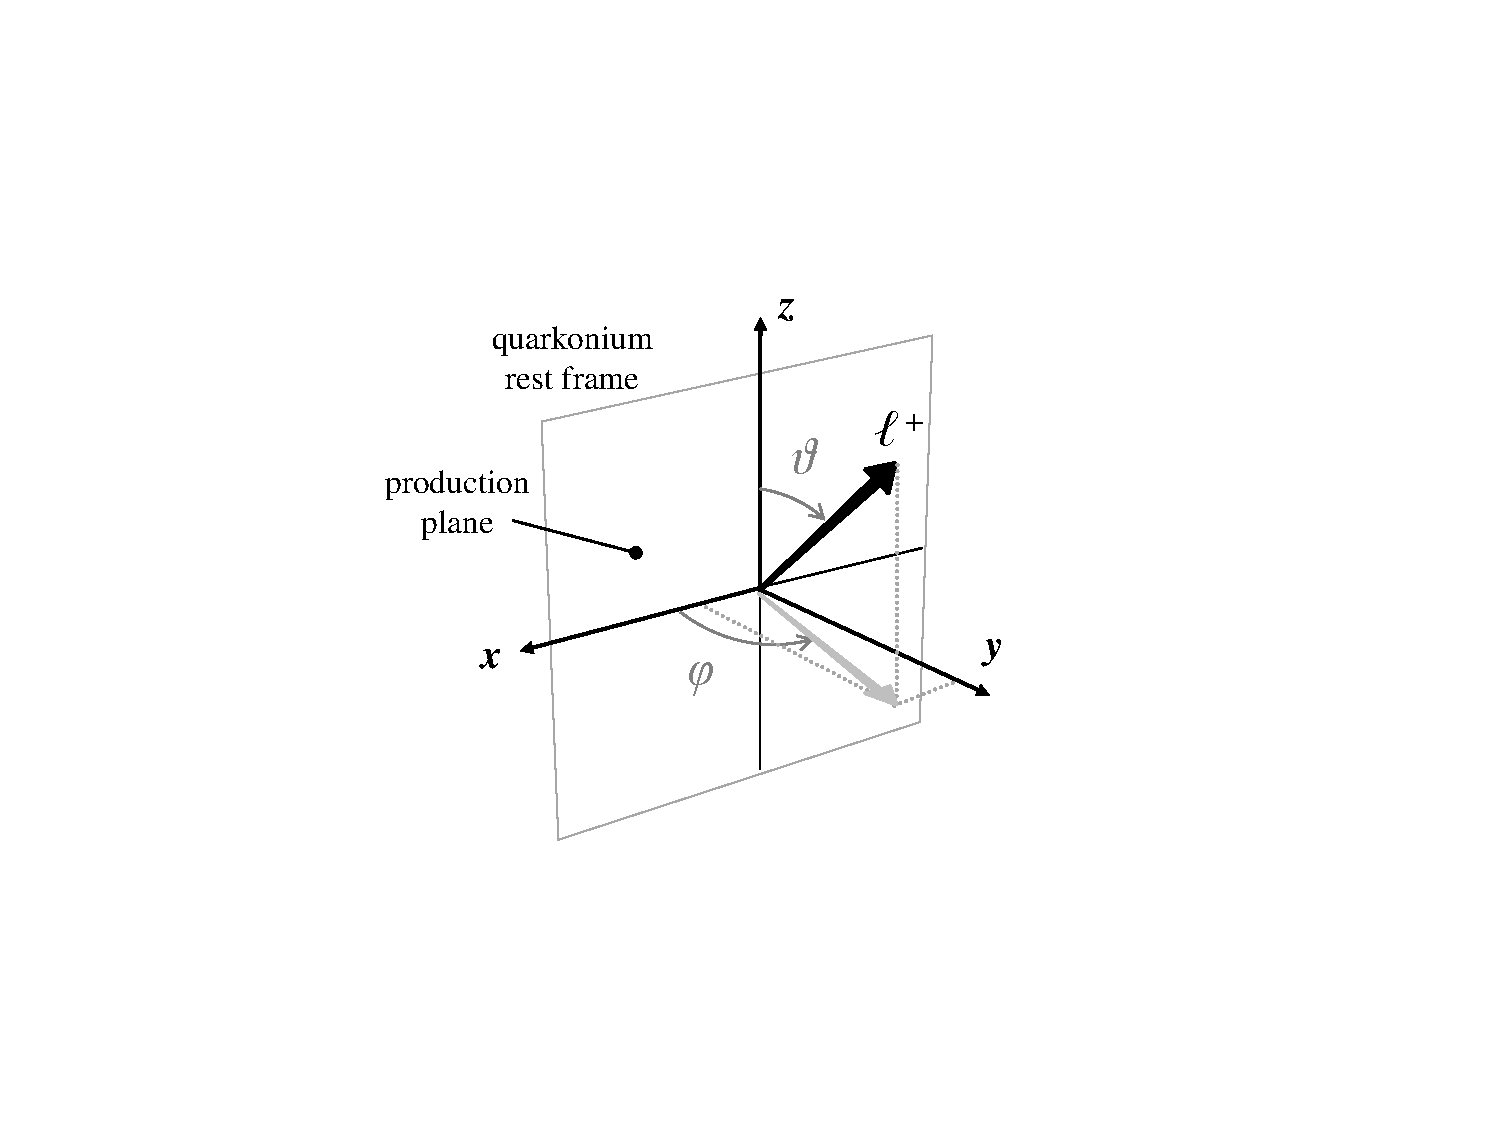
\includegraphics{Figures/chapter1/fig_coordinates_new.pdf}}
\caption{Coordinate system for the measurement of a
dilepton decay angular distribution in the quarkonium rest frame.
The $y$ axis is perpendicular to the plane containing the momenta of the colliding beams.
The choice of the definition of the polarization axis $z$ determines the measurement frame.
From Ref.~\cite{bib:Faccioli-EPJC}.}
\label{fig:coordinates}
\end{figure}

\begin{figure}[h]
\centering
\resizebox{0.8\linewidth}{!}{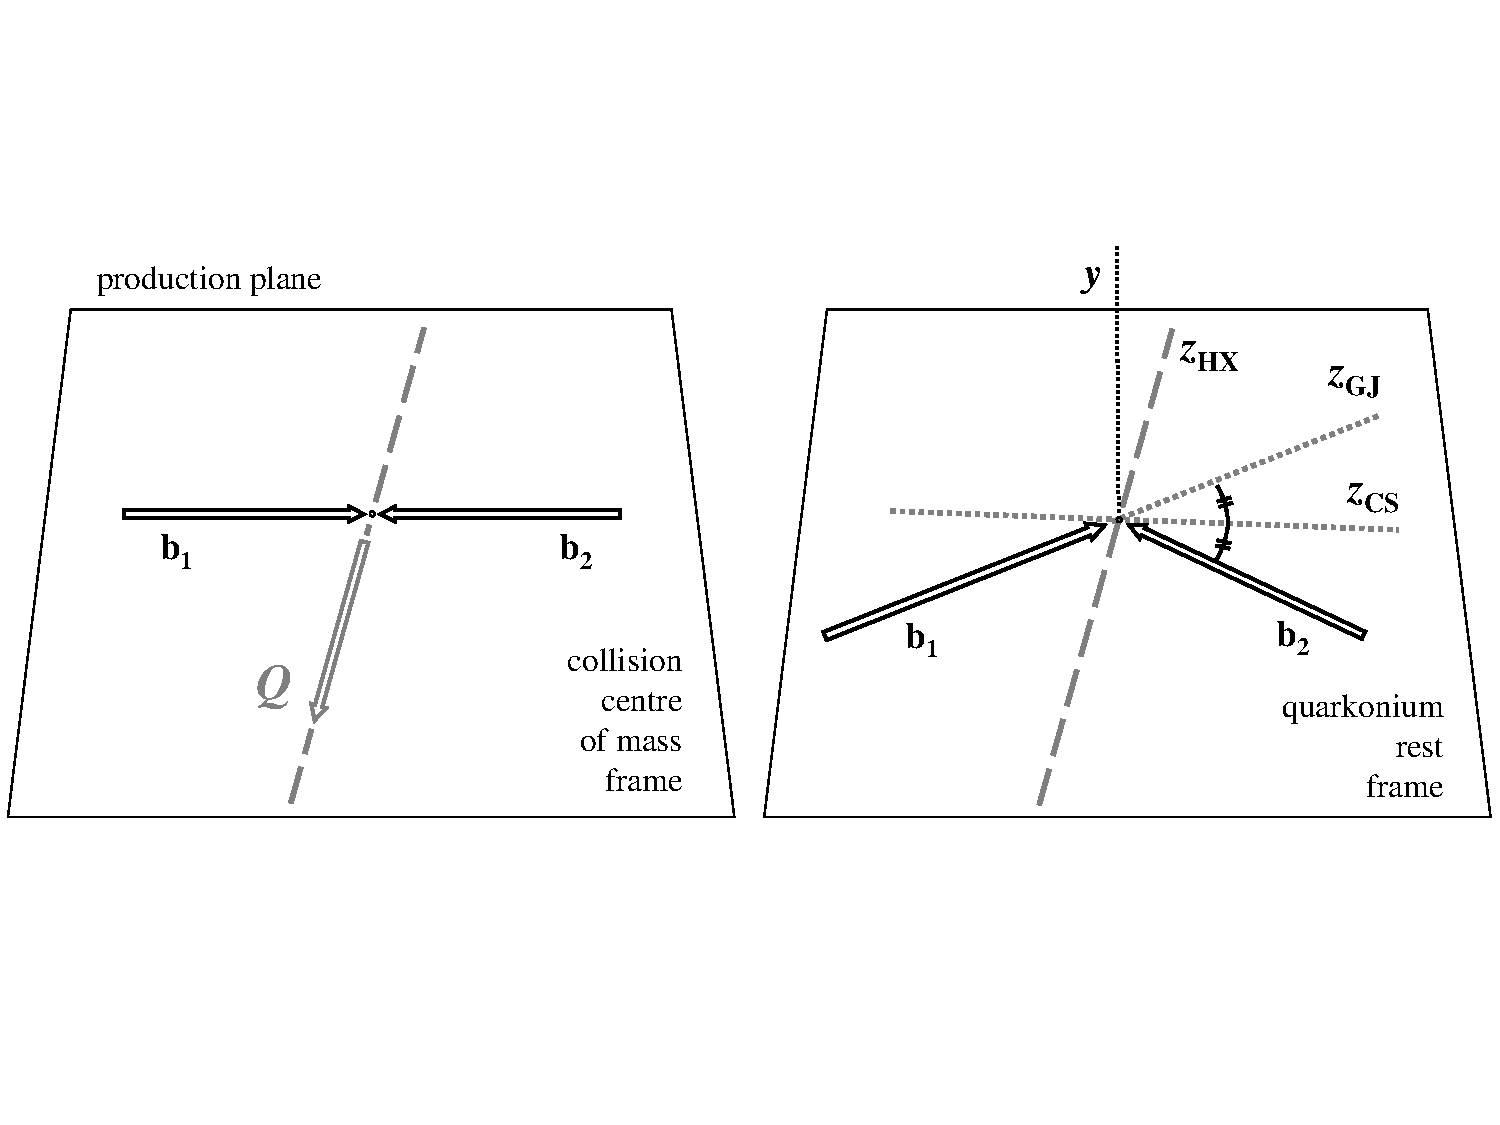
\includegraphics{Figures/chapter1/fig_frames.pdf}}
\caption{Schematic illustration of reference frames frequently used in 
studies of quarkonium production.
In this study, the polarization axis $z$ is chosen according to the HX convention. 
From Ref.~\cite{bib:Faccioli-EPJC}.}
\label{fig:frames}
\end{figure}

Given that we are studying mid-rapidity and high-\pt quarkonia,
it is very reasonable to focus the analysis by presenting the main results 
in the form of the polar anisotropy parameter, \lth,
in the centre-of-mass helicity (HX) frame,
where the $z$ axis coincides with the flight direction of the meson in
the centre-of-mass frame of the colliding hadrons, 
as illustrated in Fig.~\ref{fig:frames}.
Other anisotropy parameters offer useful crosschecks.

The polar anisotropy parameter is determined using a simplified version of
Eq.~\ref{eq:ang_distr_general}, integrating over the azimuthal decay angle,
%\begin{linenomath}
\begin{equation}
W(\costh) \propto 1+\lth \cos^2 \vartheta \; .
\label{eq:W}
\end{equation}
%\end{linenomath}
Translating this equation into words, we project the ``final analysis ntuple" into
the \costh variable, only selecting dimuons in the prompt region and in the 
\jpsi ``signal mass window", and then fit that distribution with a parabolic function
to determine \lth.

In reality, things are more complex than suggested by this simple description.
To start with, the analysis is made using the observable \abscosth, 
so as to decrease the statistical uncertainties shown in the figures.
Indeed, the symmetry of the underlying physics implies that the distribution 
must be symmetric around zero and, hence, there is no information gain in using
the \costh variable.
More importantly, the analysis is made in many \pt bins,
in order to measure the \pt dependence of \lth.
The \pt bins are relatively narrow, especially at low \pt,
not so much because we need to have 
a high granularity to determine a potential trend of \lth with \pt 
but rather to ensure that, within those bins, the variation of the polarization 
(if there is any) can be neglected.
It might be worth noting that the integration over the $|y| < 1.2$ range is 
justified by the observation that no variations of the polarization are 
expected in any theory model within that relatively narrow mid-rapidity range,
a prediction in good agreement with the results of the BPH-13-003 analysis,
which were provided in two rapidity ranges for the \jpsi meson, 
$|y| < 0.6$ and $0.6 < |y| < 1.2$.
In these conditions, we can write
Eq.~\ref{eq:W} as
%\begin{linenomath}
\begin{equation}
W(\abscosth,\pt) \propto 1+\lth(\pt) \cos^2 \vartheta \; .
\label{eq:wfit}
\end{equation}
%\end{linenomath}

A bigger challenge of the analysis is that 
we cannot use Eq.~\ref{eq:wfit} to directly fit the measured (``raw data") \costh distributions 
because they are affected by sculpting effects introduced by the limited acceptance coverage of the
detector and by the efficiencies of the trigger and reconstruction steps.
In other words, the fit must be done on distributions previously corrected for 
those experimental effects.
As in all other previous analyses, we evaluate the detection acceptance 
through a very detailed (``full") simulation of the whole detection chain, 
from the trigger step to the offline reconstruction and event selection criteria.
The Monte Carlo simulation is made assuming unpolarized production
(i.e.,\ a flat \costh distribution), so that any non-flat trends we see in 
the simulated distributions are caused by the convolution of all the 
detection effects 
(mostly the acceptance, but also the single muon and dimuon efficiencies).
So, we start by dividing (in each \pt bin) 
the measured \abscosth distribution by the simulated one, 
before we perform the fit using Eq.~\ref{eq:wfit}.
In this way, the only remaining reason for potential modulations of the angular distribution
is the polarization of the measured charmonium samples.

To probe the possible existence of a residual azimuthal anisotropy,
the analysis has been redone, in exactly the same way (same \pt bins, etc.)
replacing the $|\costh \, |$ polar angle by the $\varphi$ azimuthal angle.
The $\varphi$ distributions, corrected for acceptance as previously explained, 
are fitted with the function
%\begin{linenomath}
\begin{equation}
W(\varphi|\vec{\lambda}) \propto 1 + \beta\cos2\varphi \; ,
\label{eq:wfit-phi}
\end{equation}
%\end{linenomath}
with $\beta = (2 \, \lambda_\varphi) / (3+\lambda_\theta)$,
obtained from Eq.~\ref{eq:ang_distr_general} integrating over the polar decay angle.
